\documentclass[conference]{IEEEtran}
\IEEEoverridecommandlockouts
\usepackage{cite}
\usepackage{amsmath,amssymb,amsfonts}
\usepackage{algorithmic}
\usepackage{graphicx}
\usepackage{svg}
\graphicspath{{assets/}}
\svgpath{{assets/}}
\usepackage{textcomp}
\usepackage{xcolor}
\usepackage{booktabs}
\usepackage{multirow}
\usepackage{stfloats}
\usepackage[a4paper,left=13mm,right=13mm,top=12mm,bottom=14mm]{geometry}
\usepackage{pgfplots}
\usepgfplotslibrary{groupplots}
\pgfplotsset{compat=1.18}

\newcommand{\figureplaceholder}[2]{%
  \fbox{\parbox[c][#2][c]{0.95\linewidth}{\centering\footnotesize\bfseries #1}}%
}
\newcommand{\tableplaceholder}[2]{%
  \fbox{\parbox[c][#2][c]{0.96\textwidth}{\centering\footnotesize\bfseries #1}}%
}

\begin{document}
% Keep the figure-to-text gaps compact. IEEEtran's stretchable float glue can
% otherwise absorb most of the remaining column height on figure-heavy pages.
\setlength{\textfloatsep}{8pt}
\setlength{\dbltextfloatsep}{8pt}
\setlength{\floatsep}{6pt}
\setlength{\dblfloatsep}{6pt}

\title{A Fully Asynchronous Parallel-Path Hierarchical NoC for Scalable High-Fanout On-Chip Communication}

% Double-blind review format: author identities and affiliations are omitted.
\author{Anonymous Authors}

\maketitle
\vspace{-3em}

\begin{abstract}
As manycore processors, AI accelerators, and other large SoCs grow, their on-chip networks must carry traffic across longer distances and increasingly shared links. This scaling creates two related problems: global traffic competes for a small number of upper-level links, while one-to-many transfers send repeated copies of the same data through those links. The network therefore needs more parallel paths and in-network replication, while avoiding unnecessary copies at the source. We address this problem with a fully asynchronous hierarchical NoC. Each 64-node tile contains a three-level local tree, while independent $2\times2$ upper-mesh planes connect the tile boundaries. At each tree level, multiple routers provide several independent request/data paths, called lanes, between adjacent levels. Native multicast keeps one packet while destinations share a path and creates copies only when paths diverge. A phase-safe controller selects one lane for each packet branch and preserves the two-phase request/acknowledge protocol during the selection. Post-synthesis evaluation shows that PROP reaches 379.2~Mflit/s per NoC node in the 64-node network, 58.7\% above a flat mesh. Native multicast reduces F16M5 completion latency by 93.8\% relative to repeated unicast. In the 256-node four-tile network, PROP reaches 154.7~Mflit/s per node, 37.5\% above the flat-mesh baseline.
\end{abstract}

\begin{IEEEkeywords}
asynchronous NoC, hierarchical NoC, hardware multicast, multi-lane routing, scale-out interconnects, neuromorphic computing
\end{IEEEkeywords}

\section{Introduction}\label{sec:introduction}

Modern manycore processors, AI accelerators, and other large SoCs integrate
hundreds or thousands of processing elements and memory blocks. Within these
chips, the on-chip network determines how efficiently data moves between
compute regions. As the number of endpoints grows, packets traverse more
routers, traffic from many regions converges on shared links, and one-to-many
transfers increase replication traffic. TrueNorth integrates 4,096 neurosynaptic cores
\cite{merolla2014truenorth}, PAICORE connects 1,024 cores through a
hierarchical fabric \cite{zhong2025paicore}, and Hala Point scales 1,152
Loihi~2 processors to 140,544 cores \cite{intel2021loihi2,intel2024halapoint};
these systems illustrate how communication becomes a limiting factor as
on-chip systems scale.

Scale-out creates a path-capacity problem. Local traffic can remain within one
tile, but traffic between distant regions must share a smaller set of
upper-level links. As the number of endpoints increases, these shared links
can become congested even when local routers are lightly loaded. A scalable
NoC therefore needs several independent links between levels so that traffic
can be distributed across multiple paths. The same issue appears in dense
streaming and sparse event-driven systems; neuromorphic events provide a clear
example because a short event may reach nearby and distant destinations
\cite{moradi2018dynaps,merolla2014tree,su2025hbs}.

Fanout creates a second problem. Sending one-to-many traffic as separate
unicast packets repeats the same flit on common links, increasing injection
and queueing pressure. Widening one upper-level router can provide more
capacity, but it also makes that router handle more competing requests and
increases its control cost. The proposed design uses several parallel routers
and keeps a multicast packet shared until its destination paths diverge.

Following the standard interconnection-network model
\cite{dally2004book,krishna2013smart}, communication latency is

\begin{equation}\label{eq:latency} T_{\mathrm{comm}} = Ht_r + Ht_w + T_c + \frac{L}{b}. \end{equation}

where \(H\) is hop count, \(t_r\) and \(t_w\) are the per-hop router and link
delays, respectively, \(T_c\) is contention delay, and \(L/b\) is serialization delay.
Topology reduces \(H\) and supplies path capacity; routing distributes
load and shares multicast paths; router microarchitecture reduces local
delay and increases service rate. Existing techniques improve individual
terms through high-radix or hierarchical connectivity
\cite{kim2007flattened,zhong2025paicore}, adaptive routing and hardware
multicast \cite{xiang2017carpool,jerger2008vctm}, or wide and asynchronous
routers \cite{fischer2025floonoc,liu2026monet,zhang2026reusable}.

These topology and router choices expose different implementation tradeoffs.
Regular mesh and torus networks retain simple routers but require more hops as dimensions
grow. High-radix and hierarchical structures reduce hop count or preserve
locality, while adaptive routing and hardware multicast distribute load and
share common path segments. Wider datapaths and parallel channels increase
service rate, but a hierarchy can concentrate traffic in a few upper-level
routers and make them congested. Scale-out therefore requires distributed path
capacity, in-network replication, and control that safely coordinates parallel
physical lanes.

This paper presents a fully asynchronous parallel-path hierarchical NoC
for high-fanout communication. Its contributions are:

\begin{itemize}
\item \textbf{Parallel-path hierarchy:} multiple intermediate routers
connect several physical lanes between stages, while independent mesh
planes connect tiles. The structure preserves short local paths and
distributes converging traffic.
\item \textbf{Native hierarchical multicast:} one injected transaction
remains multicast across the hierarchy and upper meshes, replicating only
at routing branches and sharing common path segments.
\item \textbf{Phase-safe parallel-lane control:} packet-lifetime path
binding preserves two-phase request and acknowledgment state during lane
selection and arbitration without local clocks.
\end{itemize}

\section{Background and Motivation}\label{sec:background}

\subsection{Communication in Large-Scale Systems}\label{sec:large-scale-communication}

Large systems combine local traffic with less frequent global transfers.
Address-Event Representation (AER) is one concrete example: an event is a
compact address-bearing packet representing one or more neural spikes, and
one event may target multiple destination cores
\cite{moradi2018dynaps,merolla2014tree}. Thus a sparse source can still create
high-fanout transfers, routing metadata, and contention
\cite{su2025hbs}. The same distinction appears in accelerator and manycore
systems as local streams, regional synchronization, and global reductions.
Local traffic therefore needs short paths and low per-hop overhead, while
global and high-fanout traffic needs aggregate bisection capacity and
efficient replication.

The interconnect determines whether this traffic can scale. A shared bus is
simple, but every transfer passes through one arbitration point and one wire
bundle; serialization, electrical fanout, and wire length limit bandwidth as
the number of PEs increases. A NoC distributes point-to-point links and
routers, so independent transfers can reuse different links concurrently
\cite{dally2004book,krishna2013smart}. Fig.~\ref{fig:basic-concepts}(a)
shows this organization: PEs attach to local routers, which make capacity,
locality, and path diversity explicit design dimensions.

\begin{figure}[!t]
\centering
\includesvg[inkscapelatex=false,width=\columnwidth]{basic_concepts.svg}
\caption{Basic communication concepts for scalable asynchronous NoCs:
(a) PE/router connectivity, (b) four-phase bundled-data transfer, and
(c) two-phase bundled-data transfer.}
\label{fig:basic-concepts}
\end{figure}

\subsection{Scale-Out NoC Architectures}\label{sec:scaleout-bg}

Topology, routing, and router microarchitecture then determine complementary
parts of communication cost. Meshes are modular but their diameter grows
with system size; high-radix and hierarchical networks shorten paths or
exploit locality at the cost of wiring and arbitration
\cite{zhong2025paicore}. Multicast shares common path segments through
in-network replication, while bypass, parallel datapaths, and optimized
arbitration improve service capacity
\cite{merolla2014tree,bhardwaj2019cmr,su2025hbs,krishna2013smart,rasheed2014storm,fischer2025floonoc}.

Asynchronous signaling supplies the timing discipline for these links. In
bundled-data communication, the sender stabilizes the data and changes a
request; the receiver samples the data and returns an acknowledgment.
Fig.~\ref{fig:basic-concepts}(b) shows four-phase signaling, in which both
control signals return to zero before the next transfer. Fig.~\ref{fig:basic-concepts}(c)
shows the two-phase variant used here: request and acknowledgment transitions
delimit successive transfers without that reset interval. Two-phase links
therefore advance on local completion, avoid a network-wide clock, and better
tolerate router and wire-delay variation
\cite{ghiribaldi2013transition,jiang2017async14nm,zhang2026reusable}.
This reduces per-hop protocol overhead while allowing topology and routing to
scale independently. It is also the protocol basis for the phase-safe lane
binding and PhaseAdapter described in Section~\ref{sec:multilane}; the
handshake complements, rather than replaces, path capacity.

Deterministic routing provides predictable paths, whereas adaptive routing
uses path diversity to avoid heavily loaded regions. Repeated unicast sends
the same multicast data over common links; tree-based branching removes this
redundancy, but its benefit remains limited by physical path capacity.
Neither router-level optimization nor two-phase signaling can compensate for
insufficient end-to-end capacity.

Hierarchical designs are attractive because they confine nearby traffic,
but conventional aggregation progressively reduces the number of upward
resources. Increasing the lane count of a single upper router can recover
bandwidth, yet its arbitration structures must handle more competing paths.
The proposed design spreads the upward links across several routers. Each
router handles a limited number of competing requests, while the combined
structure still provides multiple paths through the hierarchy.

\subsection{Design Motivation}\label{sec:motivation}

No single layer resolves scale and fanout together: hierarchy may
concentrate traffic, multicast still needs physical capacity, and faster
routers do not remove long routes. The proposed design therefore combines
distributed parallel connectivity, cross-level multicast, and phase-safe
binding of packet branches to physical lanes (Section~\ref{sec:proposed}).

The resulting objective is a fixed-depth organization that preserves short
local routes without progressively collapsing traffic onto a few wide
upper-level routers. Multicast should remain a single transaction until a
routing decision requires replication, and each branch must retain a
stable physical lane for its packet lifetime. In an asynchronous network,
that binding must also preserve request and acknowledgment phase state
across dynamically selected paths. These requirements jointly motivate
the topology, routing, and control mechanisms described next.

\section{Proposed NoC}\label{sec:proposed}

\subsection{Parallel-Path Hierarchical Topology}\label{sec:topology}



\begin{figure}[!t]
\centering
\includesvg[inkscapelatex=false,width=0.96\columnwidth]{topology_overview.svg}
\caption{Proposed 256-node organization.}
\label{fig:topology-overview}
\end{figure}

Fig.~\ref{fig:topology-overview} shows four identical 64-core tiles.
Within each tile, 64 endpoints feed 16 L1 routers, followed by 16 L2 and
16 L3 routers and 16 mesh routers at the tile boundary. Corresponding
mesh routers from the four tiles form 16 independent \(2\times2\) planes.
The fixed-depth hierarchy keeps local traffic on short tree paths, while
replicated upper paths distribute converging and inter-tile traffic. All
four router levels use the c1p4 geometry---one child-side lane and four
parent-side lanes per logical direction---so replication raises aggregate
path capacity without concentrating all requests in one wider router.

\begin{figure}[!t]
\centering
\includesvg[inkscapelatex=false,width=\columnwidth]{topology-v3.svg}
\caption{Inter-level connectivity and upper-mesh planes.}
\label{fig:topology-connectivity}
\end{figure}

Fig.~\ref{fig:topology-connectivity}(a) and (b) expand the two local
interconnection stages. Within each quadrant \(q\), the four L1 routers
\(L1(q,i)\) are fully connected to four replicated L2 routers \(L2(q,k)\).
Each L1 can therefore select any of four upward L2 paths, while every L2
can receive from all four L1 groups in the quadrant. The second stage
regroups routers by \(k\): for each \(k\), the four \(L2(q,k)\) routers
from different quadrants connect to four \(L3(j,k)\) routers. An upward
packet first selects \(k\) at L1--L2 and then \(j\) at L2--L3, yielding
\(4\times4=16\) physical path combinations. These replicated paths retain
the logical tree hierarchy and its region-based routing semantics while
distributing traffic across separate routing elements.

Rather than further extending the hierarchy with increasingly wide
upper-level routers, the local tree terminates at L3 and distributes
global traffic over multiple mesh planes. Fig.~\ref{fig:topology-connectivity}(c)
shows the L3-to-mesh distribution. Let \(P_h\) denote the \(h\)-th parent
lane of an L3 router and \(L_k\) the \(k\)-th local attachment of a mesh router,
where \(j,h,k\in\{0,1,2,3\}\). The connection is
\(L3(j,k).P_h \leftrightarrow Mesh(j,h).L_k\). Consequently, the 16 L3
routers expose 64 tile-boundary links, distributed evenly among 16 mesh
routers; each mesh router receives four local L3 attachments through its
four local interfaces.

Fig.~\ref{fig:topology-connectivity}(d) shows the intra-mesh step.
For a fixed plane index \((j,h)\), the corresponding \(Mesh(j,h)\) router
from each tile occupies one coordinate of a \(2\times2\) mesh. Links in
that plane connect only routers with the same \((j,h)\) index across
adjacent tiles. The 256-node configuration therefore contains 16
independent planes and 64 mesh routers in total. This mapping terminates
the local tree without introducing another high-radix aggregation point:
local communication remains in the fixed-depth hierarchy, while packets
that cross tile boundaries continue through one selected upper-mesh
plane.

The capacity effect can be expressed with a cut-capacity bound.
For a region \(S\) containing \(s\) nodes in an \(N\)-node network under
uniform-random unicast traffic, the average traffic leaving \(S\) is

\begin{equation}\label{eq:cut-traffic} \Lambda_{\mathrm{out}} = s\lambda\frac{N-s}{N-1}. \end{equation}

where \(\lambda\) is the per-node injection rate. If the cut provides
\(c\) directed lanes of capacity \(C\), the sustainable injection rate is
bounded by

\begin{equation}\label{eq:cut-bound} \lambda \leq \frac{cC(N-1)}{s(N-s)}. \end{equation}

For the 64-PE local hierarchy, the 4-PE and 16-PE cuts use (c=4) and
\(c=16\) directed lanes and yield bounds of \(1.05C\) and \(1.31C\),
respectively, both above the endpoint capacity \(C\); hence, neither
hierarchical cut becomes the intrinsic bottleneck under this traffic
model. At 256 nodes, the 16-plane upper mesh provides a central-bisection
bound of \(0.498C\) using 32 directed lanes, twice that of an equal-scale
single-plane \(16 \times 16\) mesh with 16 directed lanes (\(0.249C\)).
These are structural capacity bounds rather than throughput predictions;
measured performance is evaluated in Section IV.

\subsection{Multicast Routing Across Tree and Mesh}\label{sec:multicast}

A unified rectangular destination representation is used across both
routing tiers. Each multicast packet carries
\(R_{d} = \left\lbrack x_{0},x_{1} \right\rbrack \times \left\lbrack y_{0},y_{1} \right\rbrack\),
where \(\left( x_{0},y_{0} \right)\) and \(\left( x_{1},y_{1} \right)\)
denote the two opposite corners of the destination region. At each
router \(v\), the routing logic determines a logical output mask
\(D = R\left( v,R_{d},d_{\mathrm{in}} \right)\), where \(d_{\mathrm{in}}\) is the ingress
direction and each bit of \(D\) enables one output direction.
Physical-lane selection is handled separately by the multi-lane control
in Section~\ref{sec:multilane}, allowing the same multicast packet to traverse the
Tree--Mesh hierarchy without destination rewriting or packet
regeneration.

\begin{table}[!t]
\caption{28-bit flit format used by the routing logic.}
\label{tab:flit-format}
\centering
\scriptsize
\setlength{\tabcolsep}{3.6pt}
\renewcommand{\arraystretch}{1.05}
\begin{tabular}{lcccccc}
\toprule
\textbf{Head} & \textbf{Tail} & \textbf{$y_1$} & \textbf{$x_1$} & \textbf{$y_0$} & \textbf{$x_0$} & \textbf{ID} \\
\midrule
\texttt{[27]} & \texttt{[26]} & \texttt{[25:20]} & \texttt{[19:14]} & \texttt{[13:8]} & \texttt{[7:2]} & \texttt{[1:0]} \\
\bottomrule
\end{tabular}
\end{table}

Table~\ref{tab:flit-format} summarizes the 28-bit flit format used by the
routing logic. Bits~[27] and~[26] identify Head and Tail flits. On a Head
flit, the four 6-bit coordinate fields \(y_1,x_1,y_0,x_0\) encode the two
opposite corners of the destination rectangle, while the 2-bit packet-ID
field does not participate in routing. A unicast is represented as a
degenerate rectangle with identical corners, allowing the same header to
support both point-to-point and rectangular multicast traffic.

\emph{Routing within Trees:} Within the local tree, routing is
determined by the spatial relation between the destination region and
the region represented by each router. Let \(R_{v}\) denote the region
covered by the current router \(v\), and \(R_{v}^{i}\) the region
associated with its \(i\)-th child. A child direction \(i\) is activated
whenever the destination region overlaps that child region, i.e.,
\(R_{d} \cap R_{v}^{i} \neq \varnothing\). Meanwhile, the parent
direction is activated only when \(R_{d}\) is not fully contained in
\(R_{v}\), allowing the packet to continue upward until reaching the
smallest hierarchy level that covers all destinations. The ingress
direction is excluded from the output mask to avoid immediate
backtracking. This rule is recursively applied across the three tree
levels: L1 resolves destinations at PE level, whereas L2 and L3 operate
on progressively larger spatial subregions.

\begin{center}
\begin{minipage}{0.96\columnwidth}
\hrule\vspace{2pt}
\scriptsize\textbf{Tree routing algorithm}\vspace{-2pt}
\begin{algorithmic}[1]
\STATE $D\gets\varnothing$
\FOR{each child direction $i$}
  \IF{$i\neq d_{\mathrm{in}}$ and $R_d\cap R_v^i\neq\varnothing$}
    \STATE $D\gets D\cup\{i\}$
  \ENDIF
\ENDFOR
\IF{$d_{\mathrm{in}}\neq\mathrm{parent}$ and $R_d\nsubseteq R_v$}
  \STATE $D\gets D\cup\{\mathrm{parent}\}$
\ENDIF
\STATE \textbf{return} $D$
\end{algorithmic}
\vspace{2pt}\hrule
\end{minipage}
\end{center}

\begin{figure}[t]
\centering
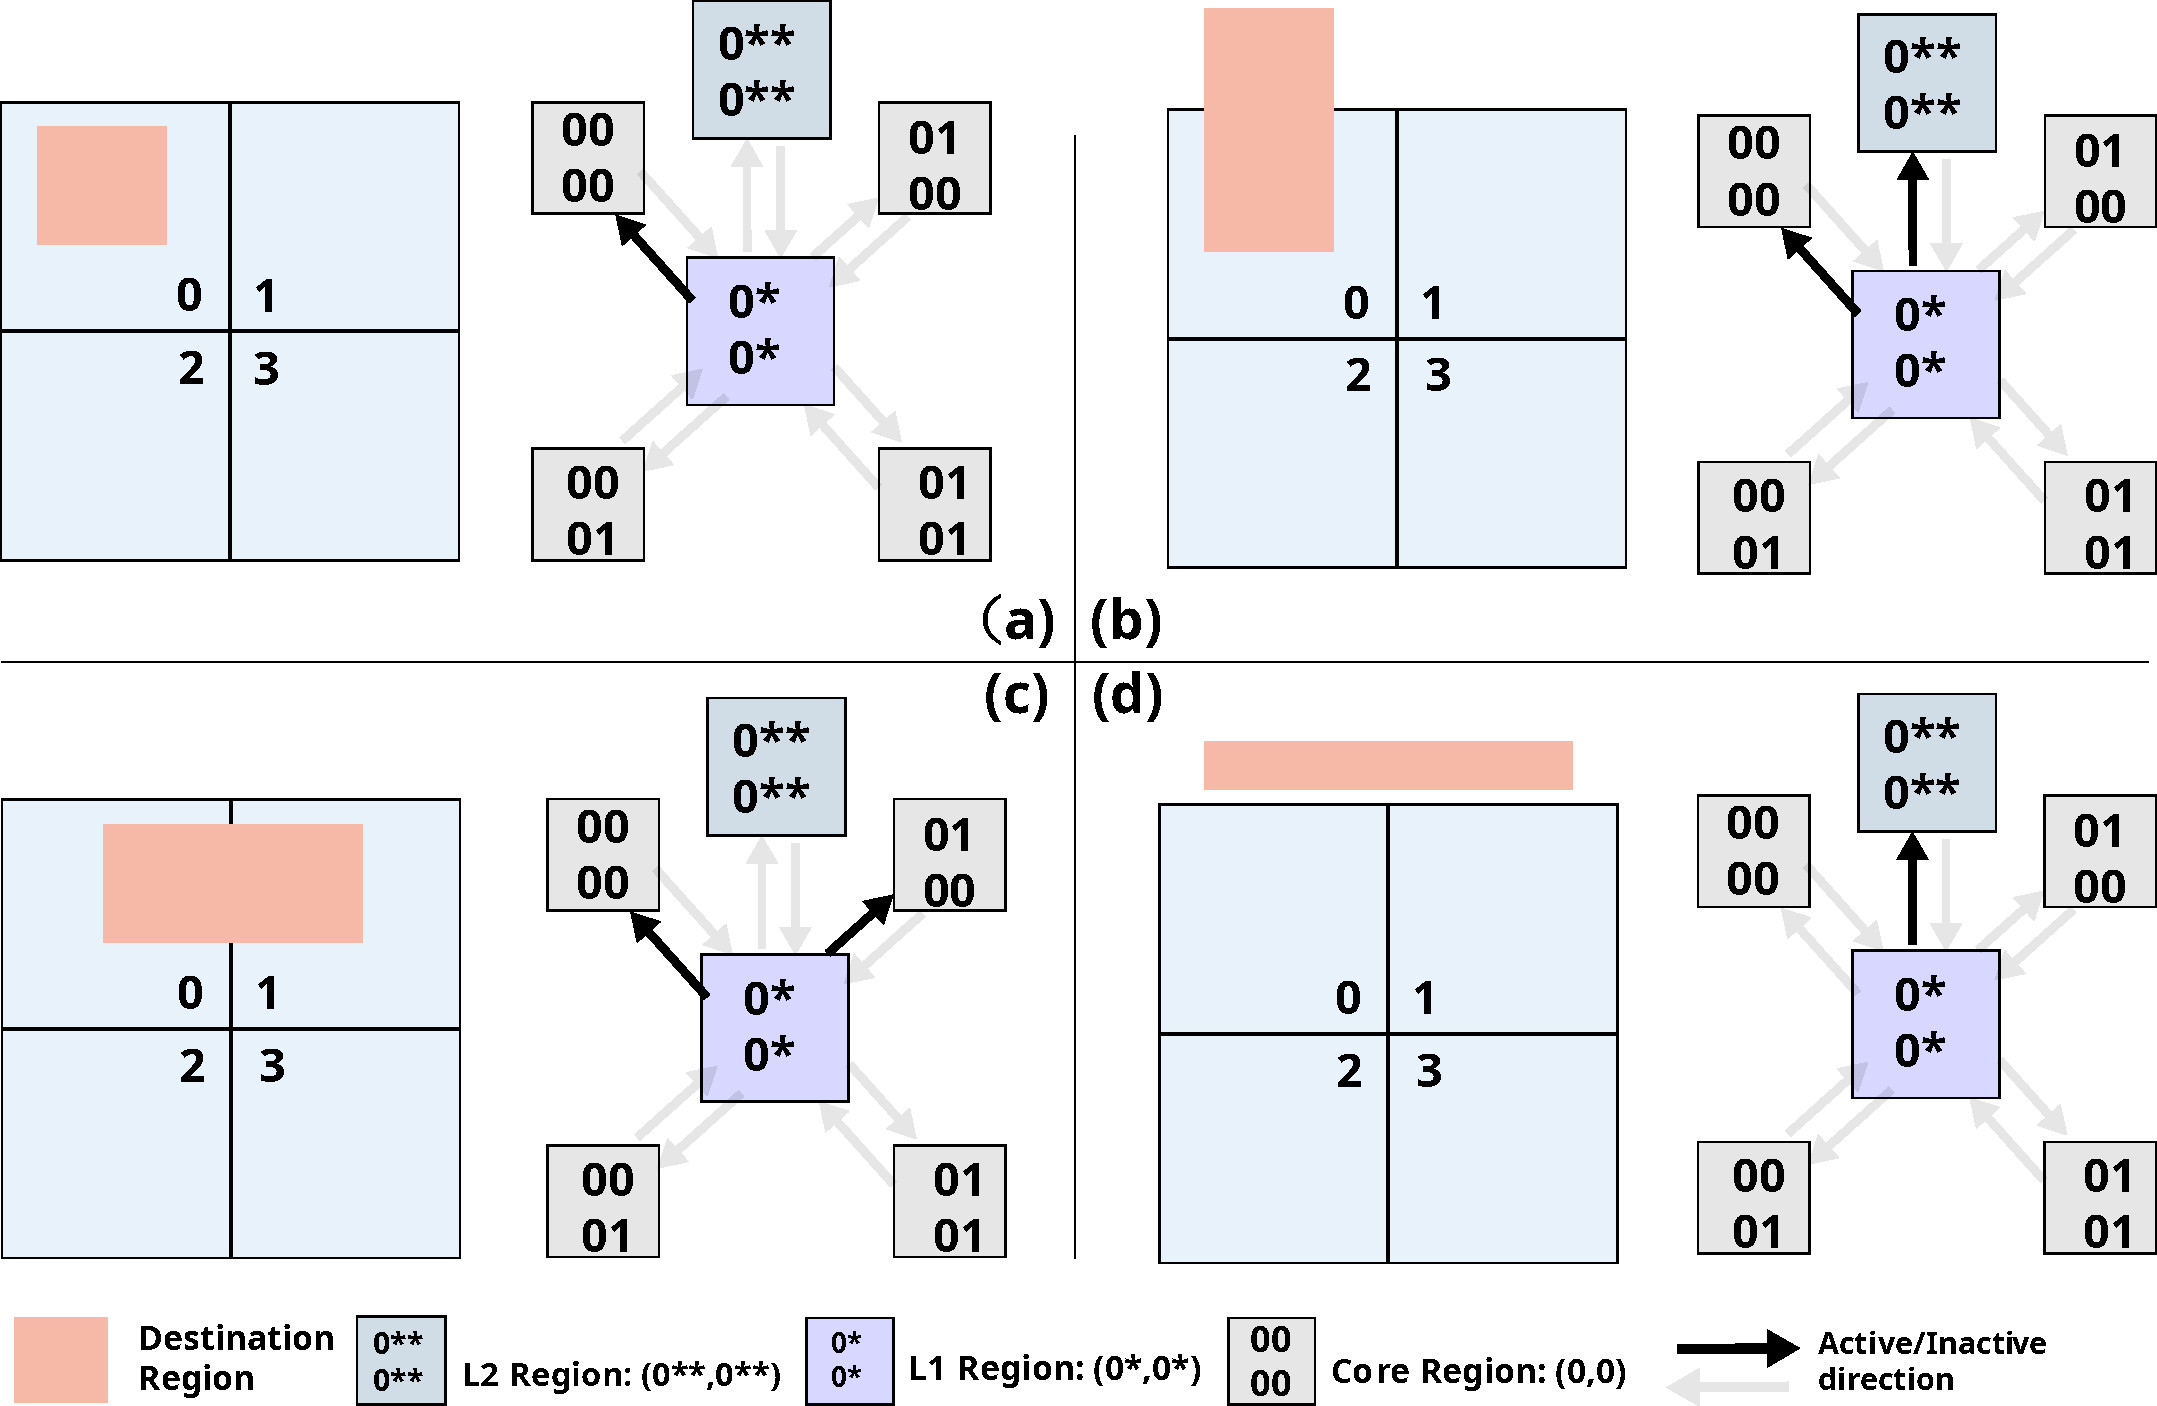
\includegraphics[width=\columnwidth]{image6.pdf}
\caption{Local-tree multicast examples for four destination regions. In (a),
the destination lies entirely in core region $(0,0)$, so the packet is sent
only to that core. In (b), the destination requires an upward transfer beyond
the current L1 region. In (c), the destination covers core regions $(0,0)$
and $(0,1)$, so both child directions are enabled. In (d), the destination
spans multiple L1 regions, so the packet is sent upward before being
replicated at the next level.}
\label{fig:tree-multicast}
\end{figure}

\emph{Routing within Mesh:}
For inter-tile communication, the
destination rectangle is projected onto the upper-mesh coordinate space.
Let
\(R_m = [x_L,x_H] \times [y_L,y_H]\), where
\(x_{L} = \lfloor\min\frac{\left( x_{0},x_{1} \right)}{8}\rfloor\),
\(x_{H} = \lfloor\max\frac{\left( x_{0},x_{1} \right)}{8}\rfloor\), and
similarly for \(y_{L}\) and \(y_{H}\). Following prior tree-based multicast routing in 2-D meshes~\cite{wang2009rpm}, a packet outside \(R_m\) is
first routed toward the nearest corner using deterministic XY routing.
Once the packet enters \(R_{m}\), it is locally delivered and replicated
only toward the remaining portions of the destination region according
to its ingress direction, as illustrated in Fig.~\ref{fig:mesh-multicast}. This approach
preserves the same destination representation across the Tree--Mesh
boundary and avoids regenerating packets for individual destination
tiles.

\begin{figure}[!t]
\centering
\includesvg[inkscapelatex=false,width=\columnwidth]{image8.svg}
\caption{Upper-mesh multicast examples for two source locations. In (a), the
source lies inside the destination region, so the packet is forwarded within
that region and branches along the required mesh directions. In (b), the
source lies outside the destination region, so the packet first reaches the
region through the shared route and then branches inside it. The dashed box
marks the destination region and the red arrows show the transmission path.}
\label{fig:mesh-multicast}
\end{figure}

\begin{figure*}[!b]
\centering
\includesvg[inkscapelatex=false,width=\textwidth]{Interconnection_v2}
\caption{Internal interconnection of the multi-lane CMR router. The input
interface computes the route mask and issues requests for eligible outputs.
The output interface arbitrates among these requests, binds each packet
branch to one physical lane, and forwards the data through the selected child
or parent path. The phase adapter preserves the request and acknowledge
phase relationship across the selected lane.}
\label{fig:router}
\end{figure*}

\begin{table*}[!t]
\caption{Node-Level Comparison With Representative Asynchronous NoC Routers}
\label{tab:router-comparison}
\centering
\scriptsize
\setlength{\tabcolsep}{4.0pt}
\renewcommand{\arraystretch}{1.05}
\resizebox{\textwidth}{!}{%
\begin{tabular}{lcccccc}
\toprule
\textbf{Design} & \textbf{Technology} & \textbf{Flit Width} & \textbf{Latency (ns)} & \textbf{Throughput$^{a}$ (Gb/s)} & \textbf{Energy$^{b}$ (pJ/bit)} & \textbf{Area ($\mu$m$^2$)} \\
\midrule
CMR~\cite{bhardwaj2019cmr} & 45 nm & 128 & 0.693$^{c}$ & -- & 0.118$^{e}$ & 54,083 \\
\cite{bertozzi2021tabula} & 40 nm & 32 & 0.980$^{d}$ & 34.24 & 0.120 & 24,866 \\
\cite{zeng2024messagebus} & 55 nm & 4 & 1.250$^{d}$ & 4.00 & 0.370 & 22,400 \\
\midrule
\textbf{This work (Async c1p4)} & \textbf{28 nm} & \textbf{28} & \textbf{1.101$^{c}$} & \textbf{84.08} & \textbf{0.0545} & \textbf{12,602} \\
\textbf{This work (Sync c1p4)} & \textbf{28 nm} & \textbf{28} & \textbf{1.000$^{c}$} & \textbf{69.99} & \textbf{0.2254} & \textbf{11,374} \\
\bottomrule
\end{tabular}%
}
\vspace{1mm}
\begin{minipage}{0.99\textwidth}
\footnotesize
$^{a}$Logical throughput. $^{b}$Energy per bit from time-based PrimeTime PX power and throughput.
$^{c}$Head-flit/head-hop latency. $^{d}$Reported average forward/flit latency.
$^{e}$CMR is derived from 75.4 pJ/(5$\times$128 bits); TaBuLA and Zeng report their values directly.
\end{minipage}
\end{table*}

% Keep the wide 64-node plot as Fig. 8 before the Part-3 single-column Fig. 7.
\setcounter{figure}{7}
\begin{figure*}[!t]
\centering
\includesvg[inkscapelatex=false,width=\textwidth]{generated_figures/NoC64Latency_Throughput.svg}
\caption{64-node unicast evaluation: (a) Bit-Complement mean flit latency,
(b) Uniform-Random mean flit latency, (c) Hotspot10 mean flit latency, and
(d) throughput versus injection rate for the three patterns.}
\label{fig:64network}
\end{figure*}

\begin{center}
\begin{minipage}{0.96\columnwidth}
\hrule\vspace{2pt}
\scriptsize\textbf{Mesh routing algorithm}\vspace{-2pt}
\begin{algorithmic}[1]
\STATE $D\gets\varnothing$; $p\gets(x,y)$
\IF{$p\notin R_m$}
  \STATE $q\gets\operatorname{nearestCorner}(p,R_m)$
  \STATE $D\gets\{\operatorname{XYNext}(p,q)\}$
\ELSE
  \IF{$d_{\mathrm{in}}\neq\mathrm{local}$} \STATE $D\gets D\cup\{\mathrm{local}\}$ \ENDIF
  \STATE $W\gets(x>x_L)$; $E\gets(x<x_H)$
  \STATE $N\gets(x_L\leq x\leq x_H)\land(y<y_H)$
  \STATE $S\gets(x_L\leq x\leq x_H)\land(y>y_L)$
  \IF{$d_{\mathrm{in}}=W$} \STATE add $E,N,S$ when their predicates hold
  \ELSIF{$d_{\mathrm{in}}=E$} \STATE add $W,N,S$ when their predicates hold
  \ELSIF{$d_{\mathrm{in}}=N$} \STATE add $S$; add $W,E$ only at $y=y_H$
  \ELSIF{$d_{\mathrm{in}}=S$} \STATE add $N$; add $W,E$ only at $y=y_L$
  \ELSE \STATE add every direction whose predicate holds
  \ENDIF
\ENDIF
\STATE remove off-grid directions; \textbf{return} $D$
\end{algorithmic}
\vspace{2pt}\hrule
\end{minipage}
\end{center}

\subsection{Multi-Lane Arbitration and Phase Adaptation}\label{sec:multilane}

\begingroup
\setlength{\parskip}{0pt}
\setlength{\emergencystretch}{1.5em}

The input interface module (IPM) receives a bundled-data channel through
\(ReqIn\), \(DataIn\), and the returning \(AckOut\), following the CMR
organization in~\cite{bhardwaj2019cmr}. The incoming flits are stored in
the five-entry CMR buffer while the route-computation unit decodes the
header in parallel. Its \(PacketPathEnable\) outputs identify every
required logical direction and remain active for the packet lifetime.
Each enabled read interface then advances an independent read pointer and
produces a \(ReqDir\)/\(DataDir\) stream, allowing multicast branches to
progress at different rates. The corresponding \(AckDir\) acknowledges
each transferred flit, whereas \(TailPass\) reports that the selected
output has consumed the tail and permits that branch to release its path.

The output interface module (OPM) merges requests for one physical output.
Candidate IPMs present \(PacketPathEnable_i\), \(Req_i\), and \(Data_i\),
as shown in Fig.~\ref{fig:router}. A mutual-exclusion arbiter grants one
candidate for the packet lifetime; the granted request latch and data
multiplexer drive \(ReqOut\) and \(DataOut\) toward the downstream
channel. \(AckIn\) is the downstream acknowledgement. After each output
transfer, it is returned only as the selected \(Ack_i\), and detection of
the transmitted tail generates the matching \(TailPass\). Thus, the IPM
decides which directions participate in a multicast, while each OPM
independently arbitrates and forwards one physical output stream.

Two arbitration levels are used. In the first level shown in
Fig.~\ref{fig:lane-adapter}, an asserted \(PPE\) allows every available
\(LaneIsEmpty_i\) to set a \(RequestHold_i\). These held requests enter
the exact-width mutex, which produces a one-hot \(LaneSelect\). Feeding
the selected bit back to the mutex input prevents the choice from
changing when lane availability changes; the selection is released only
when \(PPE\) falls at packet completion. In the second level, the OPM on
that physical lane arbitrates among competing IPMs and retains its winner
until the tail passes. Lane choice and output contention are therefore
resolved by separate arbitration points.

The Phase Adapter in Fig.~\ref{fig:lane-adapter} preserves two-phase
handshake state across this dynamic binding. Each physical lane owns an
independent \(OPMReqIn_i\) toggle, while the logical IPM branch owns one
\(IPMAckIn\) toggle. An \(IPMReqOut\) event is translated only to the
selected lane. The adapter records when that lane has actually entered
the pending state \(OPMReqIn_i\neq OPMAckOut_i\), then accepts completion
only from the same selected lane and toggles \(IPMAckIn\). This ordering
keeps lane-selection transients outside the acknowledgement event path
and prevents a stale lane phase from creating a premature or missing
completion.

\endgroup

% This single-column figure belongs to Part 3C and is Fig. 7; restore the
% counter afterward so the following wide figure remains Fig. 9.
\setcounter{figure}{6}
\begin{figure}[!t]
\centering
\includesvg[inkscapelatex=false,width=\columnwidth]{LaneSelector_PhaseAdapter}
\caption{Packet-lifetime lane selection and phase adaptation.}
\label{fig:lane-adapter}
\end{figure}
\setcounter{figure}{8}

\section{Evaluation}\label{sec:evaluation}

\subsection{Experiment Setup}\label{sec:setup}

All designs use the TSMC 28-nm HPC+ standard-cell library. Timing and performance are obtained from
MAXIMUM-SDF gate-level simulation; power and energy use time-based PrimeTime
PX analysis. All implementation metrics are post-synthesis results.

\subsection{Node-Level Evaluation}\label{sec:node-eval}

Router primitives are evaluated using cXpY notation, where X and Y denote
the child-side and parent-side lane counts per logical direction.
For network-level experiments, each case uses five-flit packets. At each
source, packet headers are generated with exponentially distributed
inter-arrival times. The five flits belonging to one packet are presented as a
packet burst, while asynchronous handshakes and router arbitration determine
their actual progress through the network. The load labels \(M5\), \(M20\),
and \(M100\) denote nominal mean injection rates of 5, 20, and
100~Mflit/s per NoC node, respectively. Since packet arrivals are sampled
from an exponential distribution, the measured injection rate of a finite
trace can differ slightly from its nominal \(M\) value.



Table~\ref{tab:router-comparison} compares the proposed router with
representative asynchronous NoCs. The Async c1p4 router sustains 84.08 Gb/s with a
1.101-ns head-hop latency and 4.581-mW post-synthesis power. Four parent-side
lanes increase service capacity while adding lane-selection and arbitration
logic; complete-network effects are evaluated next.

\subsection{Network-Level Evaluation}\label{sec:network-eval}

The complete network is evaluated at 64 nodes for topology, control, and
multicast ablations, and at 256 nodes for scale-out.

\begin{figure*}[!t]
\centering
\includesvg[inkscapelatex=false,width=\textwidth]{fig256_latency.svg}
\caption{256-node scale-out evaluation: (a) global Uniform-Random latency and throughput, (b) cross-tile fanout-16 completion latency, and (c) locality-dependent mean latency.}
\label{fig:256network}
\end{figure*}

\subsubsection{64-Node Ablation Study}

The 64-node comparison includes three topologies. Mesh is a flat
\(8\times8\) two-dimensional mesh in which each endpoint is attached to one
mesh router. FAT is the conventional fat-tree baseline, with progressively
wider connectivity toward the root. PROP is the topology
proposed in this work: 64 endpoints are organized into 16 L1 routers, 16 L2
routers, 16 L3 routers, and parallel boundary mesh routers. The tree levels
use multiple parent-side lanes to distribute traffic across independent
paths, while the boundary mesh provides the inter-region connection.

The three unicast patterns exercise different destination distributions.
Uniform-Random selects one destination uniformly from the other 63 nodes.
Bit-Complement sends each source to the node obtained by complementing its
6-bit node address. Hotspot10 selects from the other 63 nodes while assigning
a 1.10 weight to the four central nodes and a 1.00 weight to every other
node. Mesh, FAT, and PROP use the same seed, packet length, and generated
source-destination trace for each case.

Panels (a)--(d) of Fig.~\ref{fig:64network} show the latency and throughput
curves for all three traffic patterns. Under Uniform-Random traffic, PROP
reaches 379.2 Mflit/s per NoC node, which is 58.7\% higher than Mesh and
2.75$\times$ the FAT result. The same ordering appears for Bit-Complement
and Hotspot10 traffic, where PROP reaches 506.4 and 379.4 Mflit/s per NoC
node, compared with 152.2 and 237.2 for Mesh.

With identical traces, native multicast injects one packet and replicates in
network. It reduces completion latency by 94\%--98\% across F16M5, F16M20,
and F32M5, including 9.24 ns versus 148.60 ns at F16M5, as shown in
Fig.~\ref{fig:64-multicast-power}(a). At \(M100\), Async PROP uses 64.7 mW
and 13.35 pJ/flit, compared with 73.5 mW for Mesh and 284.3 mW for Sync
PROP; its mean latency is 10.33 ns versus 13.35 ns for Sync, with 11.6\%
area overhead (Fig.~\ref{fig:64-multicast-power}(b); Table~\ref{tab:async-sync-network}).

\begin{figure}[t]
\centering
\includesvg[inkscapelatex=false,width=\columnwidth]{fig64_multicast.svg}
\caption{64-node results: (a) native multicast versus repeated-unicast completion latency; (b) total network power at \(M100\).}
\label{fig:64-multicast-power}
\end{figure}

\begin{table}[t]
\caption{64-node Async/Sync results at \(M100\).}
\label{tab:async-sync-network}
\centering
\scriptsize
\setlength{\tabcolsep}{4.5pt}
\begin{tabular}{lrr}
\toprule
Metric & Async & Sync \\
\midrule
Power (mW) & 64.7 & 284.3 \\
Energy (pJ/flit) & 13.35 & 58.66 \\
Mean latency (ns) & 10.33 & 13.35 \\
Area (normalized) & 1.116 & 1.000 \\
\bottomrule
\end{tabular}
\end{table}

\subsubsection{256-Node Scale-Out Evaluation}

The 256-node configuration connects four 64-node tiles through 16 independent
\(2\times2\) upper-mesh planes and is compared with a \(16\times16\) Mesh.
Under global Uniform Random, identical five-flit traces select destinations
uniformly from the other 255 nodes. PROP reaches 154.7 Mflit/s per NoC node
versus 112.5 Mflit/s per NoC node for Mesh, a 37.5\% increase, with a later latency knee,
with the latency knee shown in Fig.~\ref{fig:256network}(a).

For fanout-16 traffic split 8+8 across adjacent tiles, native multicast
reduces completion latency by 92\% at \(M5\) and 90\% at \(M20\)
(Fig.~\ref{fig:256network}(b)). At \(M120\), increasing intra-tile locality
produces the same trend in both networks, while PROP remains 20\%--33\%
lower in mean latency across the tested probabilities (Fig.~\ref{fig:256network}(c)).

\section{Conclusion}\label{sec:conclusion}

This paper presented a fully asynchronous hierarchical NoC for scalable
high-fanout communication. The design combines a parallel-path
fixed-depth hierarchy, native Tree--Mesh multicast, and phase-safe
multi-lane control to increase path diversity without a global clock or
source-side multicast expansion. Post-synthesis results show
379.2~Mflit/s per NoC node peak throughput in the 64-node network
(10.6~Gb/s per NoC node at the 28-bit flit width), 58.7\% above a flat mesh,
while native multicast
reduces fanout-16 completion latency
by 93.8\%. A four-lane router reaches 3.00~Gflit/s aggregate throughput,
and the 256-node four-tile system reaches 37.5\% higher peak throughput
than a conventional mesh. Together, these measurements support
coordinated topology, multicast, and asynchronous control for high-fanout
traffic.

{\renewcommand{\footnotesize}{\fontsize{8}{9.2}\selectfont}
\bibliographystyle{IEEEtran}
\bibliography{references}
}

\end{document}
